%!TEX root = ../thesis.tex

\section{キャンパス内での実験方法}
本節では,実モビリティを用いたキャンパス内での実験方法について述べる．本実験では,改良したシステムの適用可能性を調査するために,実際のキャンパス環境での走行実験を行う．以下に,実験装置, 実験環境, 実験手順について述べる．

\subsection{実験装置}
実験装置には，\Fig{fig:mobility}で示したように，AI-Formulaモビリティを使用する．モビリティには，NVIDIA Jetson AGX Orinを搭載し，改良したシステムを実行するための計算資源を提供する．また，前方の環境認識のために，ステレオカメラが搭載されている．

\newpage

\subsection{実験環境}
実験環境には，千葉工業大学キャンパスの２号館周りの通路を使用する\Fig{fig:chibatech_cource}．この環境は，1周約？？？mの屋外であり，様々な照明条件や背景が存在する．また，歩行者や障害物が存在する．

\begin{figure}[H]
\centering
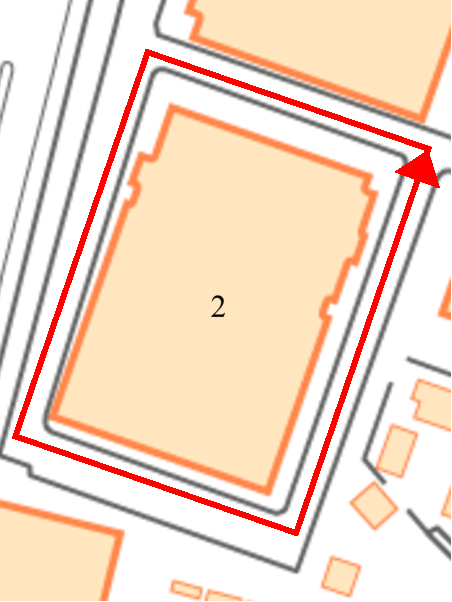
\includegraphics[width=0.8\linewidth]{images/pdf/chibatech_cource.pdf}
\caption{Experiment course around Building 2 of Chiba Institute of Technology.}
\label{fig:chibatech_cource}
\end{figure}

\subsection{実験手順}
実験手順は以下の通りである．まず，モビリティをスタート地点に配置し，ターゲットとなる被験者に対してテキストプロンプトを設定する．次に，モビリティを起動し，被験者が通路を歩行する際に，モビリティが被験者を追従するように制御する．実験中，モビリティの位置情報やカメラ映像，システムの処理ログを記録する．最後に，モビリティを停止し，データを収集する．この手順を複数回繰り返し，様々な条件下でのデータを取得する．

\newpage